\section{Performance}
Dans cette section, nous allons analyser les performances de notre application. Nous allons d'abord comparer les différentes performances des algorithmes de résolution de notre modèle. Ensuite, nous allons analyser les performances de notre application en fonction de la taille du problème.

Le problème de base que nous allons utiliser est le problème d'exemple fourni avec le projet. Il contient 2 groupes, 61 leçons, 17 profs et 19 salles.

\subsection{Comparaison des MIP}
Dans les comparaisons suivantes, le seul changement qu'il y a entre les catégories est l'algorithme de résolution utilisé. Une résolution est effectuée sur chacun des modèles et le temps de résolution est mesuré pour chacune d'entre elles.
\begin{figure}[H]
    \begin{subfigure}{0.3\linewidth}
        \centering
        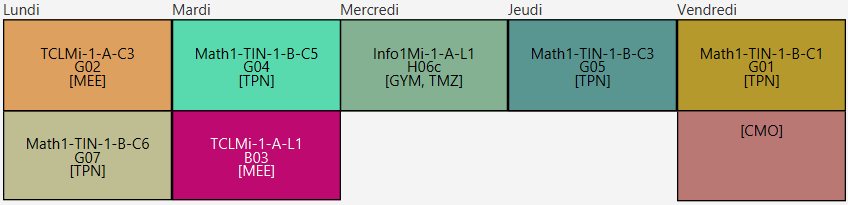
\includegraphics[width=\linewidth]{./assets/figures/perfMIP0const0_0.98.png}
        \caption{Modèle 0 - 0.98s}
    \end{subfigure}
    \hfill
    \begin{subfigure}{0.3\linewidth}
        \centering
        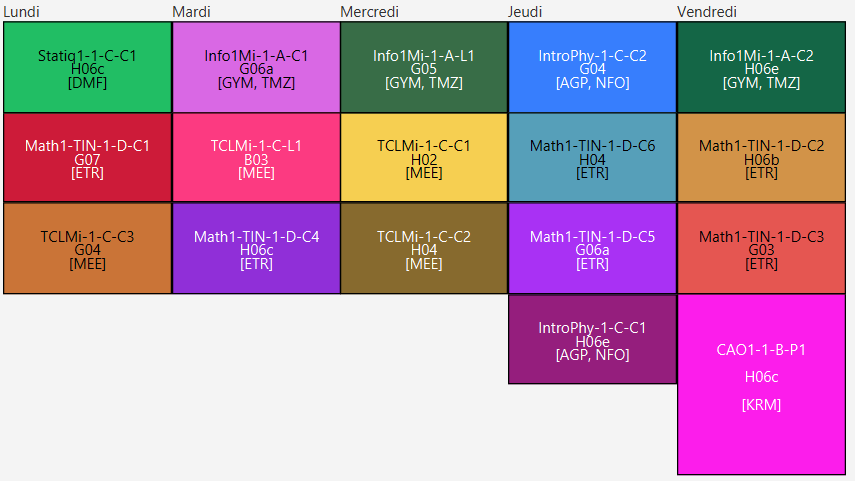
\includegraphics[width=\linewidth]{./assets/figures/perfMIP0const1_1.12.png}
        \caption{Modèle 1 - 1.12s}
    \end{subfigure}
    \hfill
    \begin{subfigure}{0.3\linewidth}
        \centering
        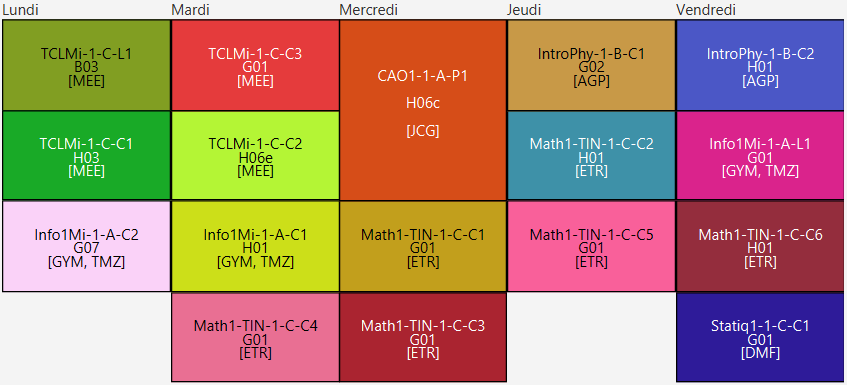
\includegraphics[width=\linewidth]{./assets/figures/perfMIP0const2_246.png}
        \caption{Modèle 2 - 4 min 6s}
    \end{subfigure}
    \caption{MIP0 - Aucune priorité}
\end{figure}

Les figures ci-dessus représentent la résolution avec un MIP-0, ce qui correspond à un algorithme de résolution sans aucune priorité. On peut voir que la différence entre le modèle 0 et le modèle 1 est très faible. Cela est dû au fait que le modèle 1 ne contient que des contraintes supplémentaires qui ne sont pas très coûteuses à résoudre. Par contre, le modèle 2 est beaucoup plus lent. La raison derrière ces différences est le fait que sans la contrainte de capacité des salles, le solveur peut placer tous les groupes dans les mêmes cours, rien n'empêche 2 groupes de suivre le même cursus, tant que les salles ont la capacité de les accueillir. Donc quand la contrainte de capacité est ajoutée, le solveur doit tester beaucoup plus de combinaisons pour trouver une réponse acceptable. Ce qui explique la différence de temps.

On peut aussi remarquer qu'il y a beaucoup moins de cours assigné au groupe dans le modèle 0 que dans le modèle 1, qui ont pourtant très peu de différence au niveau du temps. C'est dû au fait que la contrainte qu'un groupe ne peut pas avoir plusieurs cours au même moment n'est pas présente dans le modèle 0. Donc le solveur peut assigner tout les cours au même moment sans aucun souci.

Les 3 prochains algorithmes de résolution vont être comparés à celui présenté ci-dessus, étant donné que celui présenté précédemment est celui qui n'a aucune priorité et qui est donc le plus neutre.

\begin{figure}[H]
    \begin{subfigure}{0.3\linewidth}
        \centering
        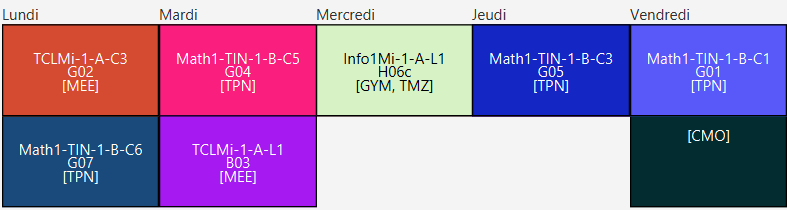
\includegraphics[width=\linewidth]{./assets/figures/perfMIP1const0_0.92.png}
        \caption{Modèle 0 - 0.92s}
    \end{subfigure}
    \hfill
    \begin{subfigure}{0.3\linewidth}
        \centering
        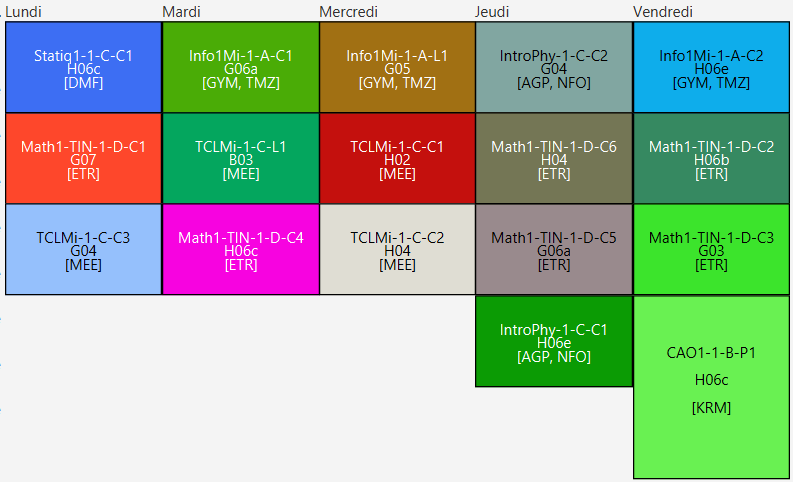
\includegraphics[width=\linewidth]{./assets/figures/perfMIP1const1_1.22.png}
        \caption{Modèle 1 - 1.22s}
    \end{subfigure}
    \hfill
    \begin{subfigure}{0.3\linewidth}
        \centering
        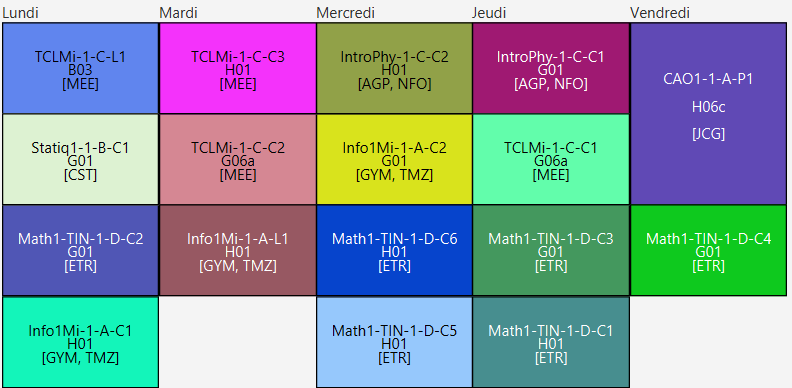
\includegraphics[width=\linewidth]{./assets/figures/perfMIP1const2_20min.png}
        \caption{Modèle 2 - Plus de 20 min}
    \end{subfigure}
    \caption{MIP1 - Solution optimale}
\end{figure}

Cet algorithme là met l'emphase sur la recherche d'une solution optimale pour notre modèle. Il va donc explorer beaucoup plus de solutions que tous les autres algorithmes et comparer toutes les solutions trouvées afin d'avoir celle qui maximise le résultat de la fonction objective. Dans les cas du modèle 0 et 1, les deux étant très basiques, le temps de résolution n'est pas beaucoup plus grand que pour l'algorithme de base. Par contre, pour le modèle 2, le temps est beaucoup plus long. Tellement long que la résolution ne se finit pas et que la limite de temps est atteinte. Cela est dû à toutes les possibilités qu'engendre la contrainte de la capacité des salles. Vu qu'elle force le modèle à assigner des cours différents aux groupes, il y a beaucoup plus de possibilités à tester, ce qui augmente grandement le temps nécessaire pour la résolution.

\begin{figure}[H]
    \begin{subfigure}{0.3\linewidth}
        \centering
        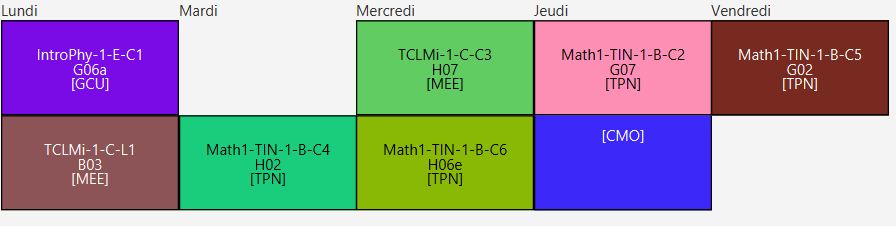
\includegraphics[width=\linewidth]{./assets/figures/perfMIP2const0_2.15.png}
        \caption{Modèle 0 - 2.15s}
    \end{subfigure}
    \hfill
    \begin{subfigure}{0.3\linewidth}
        \centering
        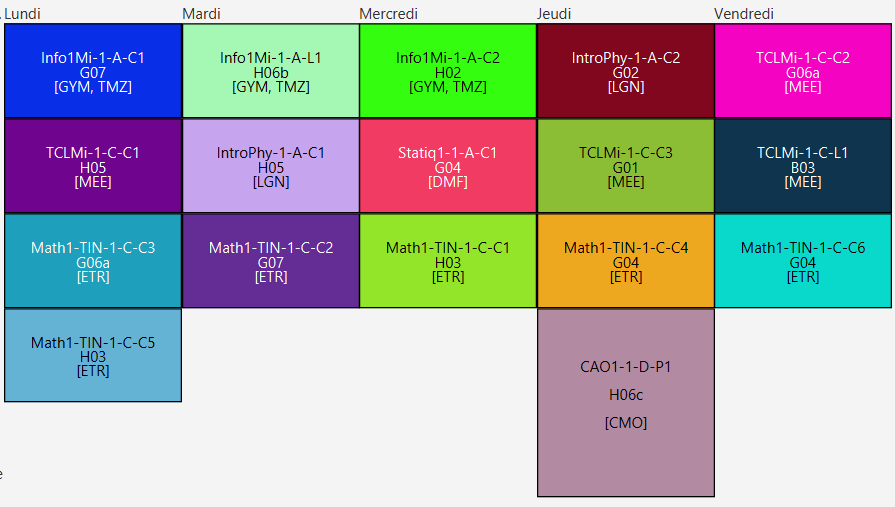
\includegraphics[width=\linewidth]{./assets/figures/perfMIP2const1_3.16.png}
        \caption{Modèle 1 - 3.16s}
    \end{subfigure}
    \hfill
    \begin{subfigure}{0.3\linewidth}
        \centering
        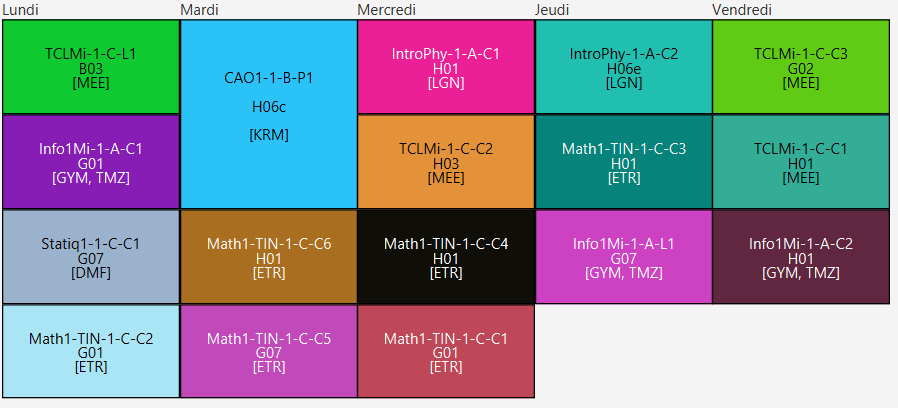
\includegraphics[width=\linewidth]{./assets/figures/perfMIP2const2_297.png}
        \caption{Modèle 2 - 4 min 57s}
    \end{subfigure}
    \caption{MIP2 - Rapidité}
\end{figure}

Cet algorithme met en avant la découverte de solutions rapidement. On remarque que le temps de résolution est plus long que pour l'algorithme de base malgré le fait que celui soit censé être le plus rapide. Ceci est dû au fait que l'algorithme standard s'arrête dès qu'il trouve une solution suffisamment proche de l'optimale. Cet algorithme va continuer d'explorer les possibilités afin de trouver le plus de solutions possibles, quel que soit leur degré d'optimisation. La preuve de cela est que dans l'algorithme de base, le solveur a retourné 2 solutions faisables, mais dans le cas de cet algorithme, ce sont 6 solutions différentes qui ont été trouvées. Dans le cas du modèle le plus long, 3 solutions de plus ont été trouvées, même si elles sont moins optimales que la solution trouvée par l'algorithme de base.

\begin{figure}[H]
    \begin{subfigure}{0.3\linewidth}
        \centering
        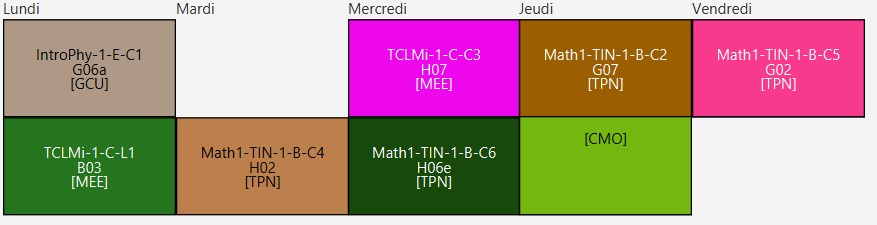
\includegraphics[width=\linewidth]{./assets/figures/perfMIP3const0_3.30.png}
        \caption{Modèle 0 - 3.30s}
    \end{subfigure}
    \hfill
    \begin{subfigure}{0.3\linewidth}
        \centering
        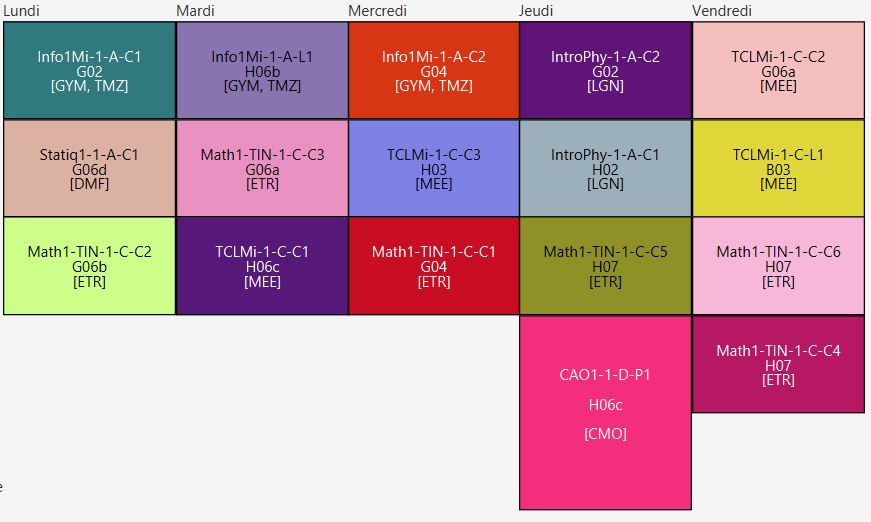
\includegraphics[width=\linewidth]{./assets/figures/perfMIP3const1_6.37.png}
        \caption{Modèle 1 - 6.37s}
    \end{subfigure}
    \hfill
    \begin{subfigure}{0.3\linewidth}
        \centering
        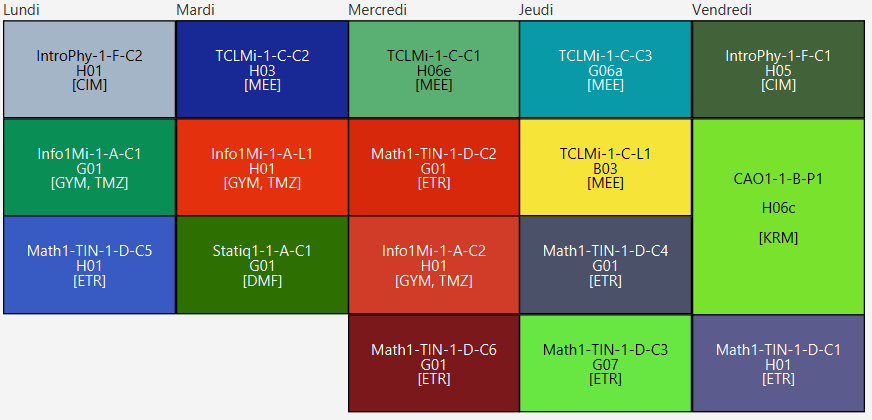
\includegraphics[width=\linewidth]{./assets/figures/perfMIP3const2_191.png}
        \caption{Modèle 2 - 3 min 11s}
    \end{subfigure}
    \caption{MIP3 - Borne inférieure}
\end{figure}

C'est le dernier algorithme mis à disposition par \textit{Gurobi}. Il cherche à améliorer la borne inférieure, c'est-à-dire, qu'il va partir de la valeur minimum pour notre fonction objective est montée petit à petit jusqu'à la valeur maximum. Cette approche permet d'obtenir rapidement une solution pour les modèles complexes, mais est par contre plus lourde pour les modèles simples. On peut remarquer ça avec les résultats obtenus pour les différentes résolutions ci-dessus. Cet algorithme est généralement utilisé pour fournir une base sur laquelle partir. Cela permet d'obtenir rapidement une solution plausible, solution que l'on fournit ensuite en tant que point de départ pour un des 3 algorithmes précédents. Cela permet de réduire leur temps d'exécution.